\documentclass[aspectratio=169,9pt]{beamer}

\usepackage[utf8]{inputenc}
\usepackage{graphicx}
\graphicspath{ {./figures/} }
\usepackage{caption}
\usepackage{subcaption}
\captionsetup{font=tiny,labelfont=tiny}
\usepackage{hyperref}
\usepackage{amsmath}
\usepackage{tikz}
\usepackage[strict]{changepage}
\usetikzlibrary{arrows,automata,positioning}
\usetheme[titleformat=smallcaps,
			sectionpage=progressbar,
			subsectionpage=progressbar,
			progressbar=frametitle,
			numbering=fraction]{metropolis}
\usecolortheme{owl}

% Information to be included in the title page:
\title{Markovian modelling of dynamic random monoallelic expression}
\author{Harshavardhan BV}
\date{\today}
\institute{IISc Bangalore}

\begin{document}
\frame{\titlepage}

\begin{frame}{Markov Model}
    \begin{columns}
        \begin{column}{0.6\textwidth}
            \begin{figure}
                \centering
                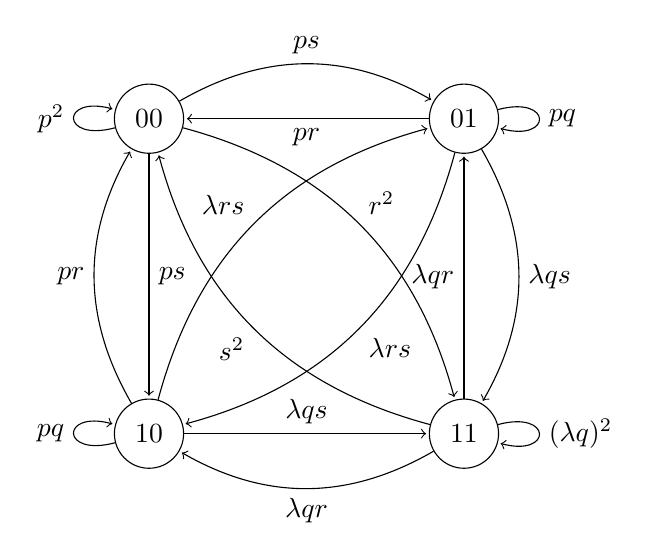
\begin{tikzpicture}[shorten >=1pt,node distance=4cm and 1cm,on grid,auto]
                    \node[state] (00)  {$00$};
                    \node[state] (01) [right of=00]  {$01$};
                    \node[state] (10) [below of=00] {$10$};
                    \node[state] (11) [below of=01] {$11$}; 
                    \path[->]
                        (00) edge [loop left] node {$p^2$}    ()
                            edge [bend left]  node {$ps$}    (01)
                            edge node {$ps$}    (10)
                            edge [bend left] node {$r^2$}    (11)
                        (01) edge [loop right] node {$pq$}    ()
                            edge node {$pr$}    (00)
                            edge [bend left] node {$\lambda rs$}    (10)
                            edge [bend left] node {$\lambda qs$}    (11)
                        (10) edge [loop left] node {$pq$}    ()
                            edge [bend left] node {$pr$}    (00)
                            edge [bend left] node {$\lambda rs$}    (01)
                            edge node {$\lambda qs$}    (11)
                        (11) edge [loop right] node {$(\lambda q)^2$}    ()
                            edge [bend left] node {$s^2$}    (00)
                            edge node {$\lambda qr$}    (01)
                            edge [bend left] node {$\lambda qr$}    (10);
                \end{tikzpicture}
                \caption{Markov State Diagram}
            \end{figure} 
        \end{column}
        \begin{column}{0.4\textwidth}
        Transition Matrix:
        \[ T =
        \begin{bmatrix}
                p^2 & pr & pr & r^2 \\
                ps & pq & \lambda rs & \lambda qr \\
                ps & \lambda rs & pq & \lambda qr \\
                s^2 & \lambda qs & \lambda qs & (\lambda q)^2 \\
        \end{bmatrix}
        \]
        At steady state
        $$ T\vec{E} = 1 \vec{E}$$
        $$ \vec{E} = \begin{bmatrix}p_{00} & p_{01} & p_{10} & p_{11} \end{bmatrix}^T$$
        \scriptsize{
        Where,
            \begin{itemize}  
                \item $\sum_j T_{ij} = 1 \quad \forall i$
                \item $\sum_i E_{i} = 1$
                \item $p$, $q$= StayOff, StayOn rate
                \item $r$, $s$  = Off, On rate
                \item $\lambda$ = Interaction Parameter
            \end{itemize}}
        \end{column}
    \end{columns}
\end{frame}

\begin{frame}{Preliminary Results}
    \begin{figure}[h]
        \begin{adjustwidth}{-5cm}{-5cm}
          \centering
          \begin{subfigure}[b]{0.33\textwidth}
            \centering
            \includegraphics[width=\textwidth]{loguni-p2vp0-classified.pdf}
            \caption{$p_2$ vs $p_0$}
          \end{subfigure}
          \begin{subfigure}[b]{0.66\textwidth}
            \centering
            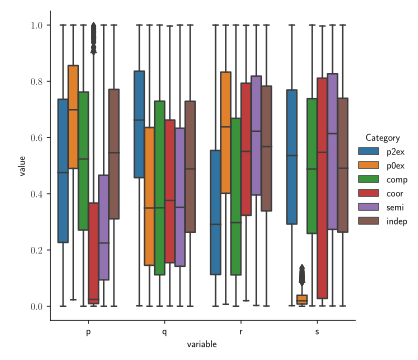
\includegraphics[width=\textwidth]{loguni-parms.pdf}
            \caption{Parameters}
          \end{subfigure}
        \end{adjustwidth}
        \caption{When $\lambda$ sampled log-uniformly}
      \end{figure}
\end{frame}

\begin{frame}{Preliminary Results}
    \begin{figure}[h]
        \begin{adjustwidth}{-5cm}{-5cm}
          \centering
          \begin{subfigure}[b]{0.33\textwidth}
            \centering
            \includegraphics[width=\textwidth]{uni-p2vp0-classified.pdf}
            \caption{$p_2$ vs $p_0$}
          \end{subfigure}
          \begin{subfigure}[b]{0.66\textwidth}
            \centering
            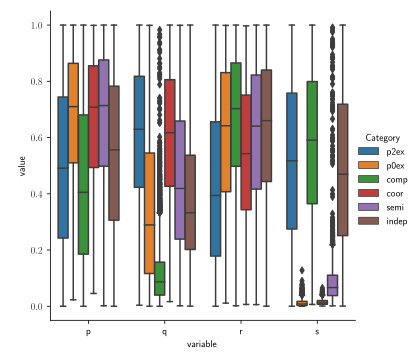
\includegraphics[width=\textwidth]{uni-parms.pdf}
            \caption{Parameters}
          \end{subfigure}
        \end{adjustwidth}
        \caption{When $\lambda$ sampled uniformly}
      \end{figure}
\end{frame}
\end{document}